% -*- TeX -*-
\documentclass{beamer}

\usepackage{tikz}
\usetikzlibrary{shapes,calc}

\title{Crustal Deformation Modeling Workshop}
\subtitle{}
\author{Brad Aagaard}
\institute{
\includegraphics[scale=0.4]{../../logos/cig_blackfg}}
\date{June 20, 2012}


% ---------------------------------------------------- CUSTOMIZATION
\newcommand{\thispdfpagelabel}[1]{}
\newcommand{\important}[1]{{\bf\color{red}#1}}
\usetheme{CIG}

% --------------------------------------------------------- DOCUMENT
\begin{document}

% ------------------------------------------------------------ SLIDE
\maketitle

% ========================================================== SECTION
\section{Introduction}
\subsection{Agenda}

% ------------------------------------------------------------- LOGO
\logo{
\includegraphics[height=4.5ex]{../../logos/cig_blackfg}}

% ------------------------------------------------------------ SLIDE
\begin{frame}
  \frametitle{Overview of Workshop}
  \summary{Draft agenda posted on geodynamics.org}
  
  \definecolor{yellow}{rgb}{1.0, 1.0, 0.45} % 255/255/115
\definecolor{dkyellow}{rgb}{0.9, 0.9, 0.0} % % 230/230/0

\definecolor{ltorange}{rgb}{1.0, 0.74, 0.41} % 255/188/105
\definecolor{orange}{rgb}{0.96, 0.50, 0.0} % 246/127/0

\definecolor{ltred}{rgb}{1.0, 0.25, 0.25} % 255/64/64
\definecolor{red}{rgb}{0.79, 0.00, 0.01} % 201/0/3

\definecolor{ltpurple}{rgb}{0.81, 0.57, 1.00} % 206/145/255
\definecolor{purple}{rgb}{0.38, 0.00, 0.68} % 97/1/175

\definecolor{ltblue}{rgb}{0.2, 0.73, 1.0} % 51/187/255
\definecolor{blue}{rgb}{0.12, 0.43, 0.59} % 30/110/150

\definecolor{ltltgreen}{rgb}{0.7, 1.00, 0.7} % 96/204/14
\definecolor{ltgreen}{rgb}{0.37, 0.80, 0.05} % 96/204/14
\definecolor{green}{rgb}{0.23, 0.49, 0.03} % 59/125/8
  
\definecolor{dkslate}{rgb}{0.18, 0.21, 0.28} % 47/53/72
\definecolor{mdslate}{rgb}{0.45, 0.50, 0.68} % 114/127/173
\definecolor{ltslate}{rgb}{0.85, 0.88, 0.95} % 216/225/229


\tikzstyle{days} = [rectangle, 
                    text width=15mm,
                    text centered,
                    minimum height=2em,
                    thin,
                    font=\bfseries,
                    draw=dkyellow!80!black,
                    top color=yellow,
                    bottom color=dkyellow]
\tikzstyle{admin} = [rectangle, 
                      draw=orange!80!black,
                      top color=ltorange!50!white,
                      bottom color=orange]
\tikzstyle{tutorial} = [rectangle, 
                      draw=green!80!black,
                      top color=ltgreen!20!white,
                      bottom color=green]
\tikzstyle{break} = [rectangle, 
                      draw=blue!80!black,
                      top color=ltblue!20!white,
                      bottom color=blue]
\tikzstyle{talk} = [rectangle, 
                      draw=ltred!80!black,
                      top color=ltred!20!white,
                      bottom color=red!70!white!100]
\tikzstyle{tinker} = [rectangle, 
                      draw=ltpurple!80!black,
                      top color=ltpurple!20!white,
                      bottom color=purple!70!white!100]

\begin{center}
\begin{tikzpicture}[scale=0.75, transform shape,
  node distance=6.0em,
  thick]

% Reference points
\coordinate (o1) at (0mm,0mm);
\coordinate (o2) at (+25mm,0mm);
\coordinate (o3) at (+50mm,0mm);
\coordinate (o4) at (+75mm,0mm);
\coordinate (o5) at (+100mm,0mm);


  % Days
  \node[days] (mon) at ($(o1)+(8.5mm,0mm)$) {Mon};
  \node[days] (tue) at ($(o2)+(8.5mm,0mm)$) {Tue};
  \node[days] (wed) at ($(o3)+(8.5mm,0mm)$) {Wed};
  \node[days] (thu) at ($(o4)+(8.5mm,0mm)$) {Thu};
  \node[days] (fri) at ($(o5)+(8.5mm,0mm)$) {Fri};

  % Morning/Afternoon
  %\node[days] (am) {Morning};
  %\node[days] (pm) {Afternoon};

  % Mon
  \path[break] ($(o1)+(0mm,-5mm)$) rectangle ++(17mm,-3.57mm); % breakfast
  \path[admin] ($(o1)+(0mm,-8.57mm)$) rectangle ++(17mm,-1.79mm); % intro
  \path[tutorial] ($(o1)+(0mm,-10.36mm)$) rectangle ++(17mm,-5.36mm); % relax 45min
  \path[tutorial] ($(o1)+(0mm,-15.72mm)$) rectangle ++(17mm,-3.57mm); % pylith 30min
  \path[tutorial] ($(o1)+(0mm,-19.29mm)$) rectangle ++(17mm,-3.57mm); % cubit 30min

  \path[break] ($(o1)+(0mm,-22.86mm)$) rectangle ++(17mm,-1.79mm); % break 15min

  \path[tutorial] ($(o1)+(0mm,-24.65mm)$) rectangle ++(17mm,-14.29mm); % pylith 2hrs

  \path[break] ($(o1)+(0mm,-38.94mm)$) rectangle ++(17mm,-5.36mm); % lunch 45min
  \path[tinker] ($(o1)+(0mm,-44.30mm)$) rectangle ++(17mm,-10.71mm); % tinker 90min
  \path[break] ($(o1)+(0mm,-55.01mm)$) rectangle ++(17mm,-3.57mm); % break 30min

  \path[tutorial] ($(o1)+(0mm,-58.58mm)$) rectangle ++(17mm,-10.71mm); % pylith 90min
  \path[tutorial] ($(o1)+(0mm,-69.29mm)$) rectangle ++(17mm,-5.36mm); % relax 45min
  \path[tinker] ($(o1)+(0mm,-74.65mm)$) rectangle ++(17mm,-5.36mm); % tinker 45min

  % Tue
  \path[break] ($(o2)+(0mm,-5mm)$) rectangle ++(17mm,-3.57mm); % breakfast
  \path[admin] ($(o2)+(0mm,-8.57mm)$) rectangle ++(17mm,-0.60mm); % intro 5min
  \path[tutorial] ($(o2)+(0mm,-9.17mm)$) rectangle ++(17mm,-10.71mm); % cubit 85min
  \path[tutorial] ($(o2)+(0mm,-19.29mm)$) rectangle ++(17mm,-5.36mm); % pylith 45min

  \path[break] ($(o2)+(0mm,-24.65mm)$) rectangle ++(17mm,-1.79mm); % pylith 15min

  \path[tutorial] ($(o2)+(0mm,-26.44mm)$) rectangle ++(17mm,-3.57mm); % pylith 30min
  \path[tutorial] ($(o2)+(0mm,-30.00mm)$) rectangle ++(17mm,-7.14mm); % pylith 60min

  \path[break] ($(o2)+(0mm,-37.14mm)$) rectangle ++(17mm,-7.14mm); % lunch 60min
  \path[tinker] ($(o2)+(0mm,-44.28mm)$) rectangle ++(17mm,-10.71mm); % tinker 90min
  \path[break] ($(o2)+(0mm,-54.99mm)$) rectangle ++(17mm,-3.57mm); % break 30min

  \path[tutorial] ($(o2)+(0mm,-58.56mm)$) rectangle ++(17mm,-12.50mm); % pylith 105min
  \path[tinker] ($(o2)+(0mm,-71.06mm)$) rectangle ++(17mm,-8.93mm); % tinker 75min

  % Wed
  \path[break] ($(o3)+(0mm,-5mm)$) rectangle ++(17mm,-3.57mm); % breakfast 30min
  \path[admin] ($(o3)+(0mm,-8.57mm)$) rectangle ++(17mm,-3.57mm); % intro 30min
  \path[talk] ($(o3)+(0mm,-12.14mm)$) rectangle ++(17mm,-3.57mm); % posters 30min

  \path[break] ($(o3)+(0mm,-15.71mm)$) rectangle ++(17mm,-3.57mm); % break 30min

  \path[talk] ($(o3)+(0mm,-19.28mm)$) rectangle ++(17mm,-7.14mm); % talk 60min
  \path[talk] ($(o3)+(0mm,-26.42mm)$) rectangle ++(17mm,-7.14mm); % talk 60min

  \path[admin] ($(o3)+(0mm,-33.56mm)$) rectangle ++(17mm,-3.57mm); % shuttle 30min
  \path[break] ($(o3)+(0mm,-37.13mm)$) rectangle ++(17mm,-7.14mm); % lunch 60min
  \path[tinker] ($(o3)+(0mm,-44.27mm)$) rectangle ++(17mm,-10.71mm); % tinker 90min
  \path[break] ($(o3)+(0mm,-54.99mm)$) rectangle ++(17mm,-3.57mm); % break 30min

  \path[talk] ($(o3)+(0mm,-58.55mm)$) rectangle ++(17mm,-7.14mm); % talk 60min
  \path[talk] ($(o3)+(0mm,-65.69mm)$) rectangle ++(17mm,-7.14mm); % talk 60min

  \path[talk] ($(o3)+(0mm,-72.83mm)$) rectangle ++(17mm,-7.14mm); % talk 60min

  % Thu
  \path[break] ($(o4)+(0mm,-5mm)$) rectangle ++(17mm,-3.57mm); % breakfast 30min
  \path[talk] ($(o4)+(0mm,-8.57mm)$) rectangle ++(17mm,-7.14mm); % talk 60min
  \path[talk] ($(o4)+(0mm,-15.71mm)$) rectangle ++(17mm,-7.14mm); % talk 60min

  \path[break] ($(o4)+(0mm,-22.85mm)$) rectangle ++(17mm,-1.79mm); % break 15min

  \path[talk] ($(o4)+(0mm,-24.64mm)$) rectangle ++(17mm,-1.79mm); % talk 15min
  \path[talk] ($(o4)+(0mm,-26.43mm)$) rectangle ++(17mm,-3.57mm); % discuss 30min

  \path[tinker] ($(o4)+(0mm,-30.00mm)$) rectangle ++(17mm,-7.14mm); % tour 60min

  \path[break] ($(o4)+(0mm,-37.13mm)$) rectangle ++(17mm,-7.14mm); % lunch 60min
  \path[admin] ($(o4)+(0mm,-44.27mm)$) rectangle ++(17mm,-7.14mm); % tour 60min
  \path[tinker] ($(o4)+(0mm,-51.41mm)$) rectangle ++(17mm,-3.57mm); % tinker 30min
  \path[break] ($(o4)+(0mm,-54.99mm)$) rectangle ++(17mm,-3.57mm); % break 30min

  \path[talk] ($(o4)+(0mm,-58.55mm)$) rectangle ++(17mm,-7.14mm); % talk 60min

  \path[tinker] ($(o4)+(0mm,-65.69mm)$) rectangle ++(17mm,-14.28mm); % tinker 60min

  % Fri
  \path[break] ($(o5)+(0mm,-5mm)$) rectangle ++(17mm,-3.57mm); % breakfast 30min
  \path[talk] ($(o5)+(0mm,-8.57mm)$) rectangle ++(17mm,-7.14mm); % talk 60min
  \path[talk] ($(o5)+(0mm,-15.71mm)$) rectangle ++(17mm,-7.14mm); % talk 60min

  \path[break] ($(o5)+(0mm,-22.85mm)$) rectangle ++(17mm,-3.57mm); % break 30min

  \path[talk] ($(o5)+(0mm,-26.42mm)$) rectangle ++(17mm,-7.14mm); % talk 60min
  \path[admin] ($(o5)+(0mm,-33.56mm)$) rectangle ++(17mm,-3.57mm); % wrapup 30min

  \path[break] ($(o5)+(0mm,-37.13mm)$) rectangle ++(17mm,-7.14mm); % lunch 60min
  \path[tinker] ($(o5)+(0mm,-44.27mm)$) rectangle ++(17mm,-28.57mm); % tinker 4hrs

\end{tikzpicture}
\end{center}



\end{frame}


% ------------------------------------------------------------ SLIDE
\begin{frame}
  \frametitle{Logistics}
  \summary{Wireless: CSMGuest, Username: guest-cfem, Password: 6jjcrjnm}

  \begin{itemize}
  \item Reimbursement forms will be distributed via email
  \item Meals
    \begin{itemize}
    \item Breakfast and lunch provided (Mon-Fri)
    \item Dinner on your own
    \end{itemize}
 \item Posters
    \begin{itemize}
    \item Introductions
      \begin{itemize}
      \item 1 slide as PDF file
      \item Put on USB memory stick or email to {\bfseries\tt baagaard@usgs.gov}
      \end{itemize}
    \item Put up your posters at lunch (or before)
    \end{itemize}
  \end{itemize}

\end{frame}

% ========================================================== SECTION
\section{CIG}
\subsection{Overview}

% ------------------------------------------------------------ SLIDE
\begin{frame}
  \frametitle{What is CIG?}
  \summary{Computational Infrastructure for Geodynamics
    ({\tt www.geodynamics.org})}
 
  \vfill

  Objective: Develop, support, and disseminate software for the
  geodynamics community.

  \vfill

  \begin{itemize}
  \item Coordinated effort to develop reusable, well-documented,
    open-source geodynamics software
  \item Strategic partnerships with the larger world of
    computational science and geoinformatics
  \item Specialized training and workshops for both geodynamics and
    larger Earth-science communities
  \end{itemize}

  \vfill
 
  Underlying principle: Earth scientists need help from computational
  scientists to develop state-of-the-art modeling codes

\end{frame}


% ------------------------------------------------------------ SLIDE
\begin{frame}
  \frametitle{CIG: Institution-Based Organization}
  \summary{Educational and not-for-profit organization}
 
  \begin{itemize}
  \item {\bf Open-organization}
    \begin{itemize}
    \item Any institution seeking to collaborate on the development of
      open-source geodynamics software
    \item No cost or size requirements
    \end{itemize}
  \item Current members
    \begin{itemize}
    \item 52 member institutions
    \item 12 foreign affiliates
    \end{itemize}
  \item NSF funding Jul 2010 -- Jun 2015
 \end{itemize}
\end{frame}


% ========================================================== SECTION
\section{CIG}
\subsection{Organization}

% ------------------------------------------------------------ SLIDE
\begin{frame}
  \frametitle{CIG Working Groups}
  \summary{Organized by sub-disciplines}
 
 \begin{itemize}
 \item Short-term crustal dynamics
 \item Long-term tectonics
 \item Mantle convection
 \item Computational seismology
 \item Geodynamo
 \item Magma dynamics
 \end{itemize}

\end{frame}


% ------------------------------------------------------------ SLIDE
\begin{frame}
  \frametitle{Short-Term Tectonics Working Group}
  \summary{}
 
 \vfill
 
 \textbf{Objective}: Simulate crustal deformation across spatial
 scales from $1$ m to $10^3$ km and temporal scales ranging from
 $0.01$ s to $10^5$ years.

 \vfill
 \begin{itemize}
 \item Formed through efforts by Brad Hager and Mark Simons before CIG started
 \item Deep roots with SCEC Stress and Deformation Over Time (SDOT) focus group
 \item Building connections with SCEC Fault and Rupture Mechanics (FARM) focus group
 \end{itemize}
\vfill

\end{frame} 


% ========================================================== SECTION
\section{CIG}
\subsection{Activities}

% ------------------------------------------------------------ SLIDE
\begin{frame}
  \frametitle{CIG Activities}
  \summary{}

  \begin{itemize}
  \item Software development: primary activity
  \item Workshops
    \begin{itemize}
    \item Sponsors workshops organized by one or more working groups
    \item Holds workshops focusing on scientific computing and geodynamics
    \end{itemize}
  \item Training in use of CIG software
    \begin{itemize}
    \item Tutorials at workshops
    \item Specialized training sessions (like this one)
    \end{itemize}
  \item Web site: {\tt geodynamics.org}
    \begin{itemize}
    \item Distribution of software and documentation
    \item Mailing lists for each working group
    \item Wiki-like web pages for community involvement
    \end{itemize}
  \end{itemize}
 
\end{frame}


% ------------------------------------------------------------ SLIDE
\begin{frame}
  \frametitle{CIG Software}
  \summary{}

  \vfill
  \begin{center}
    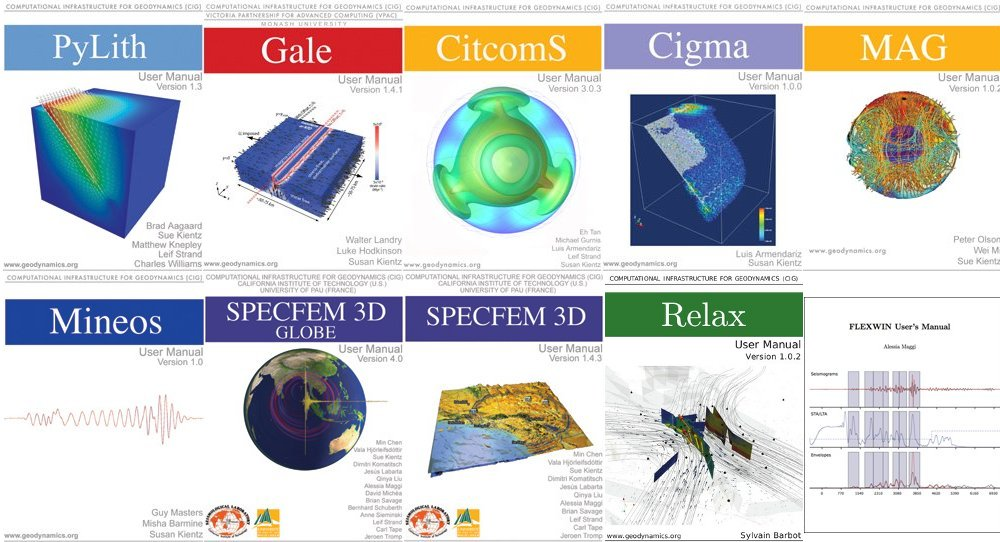
\includegraphics[width=4.5in]{figs/covers}
  \end{center}
  \vfill

\end{frame}

% ======================================================================
\end{document}


% End of file
